\documentclass[a4paper,12pt,answers]{article}

\usepackage[margin=0.75in]{geometry}
\pagenumbering{arabic}

\usepackage{amsmath, amsthm, amsfonts, amssymb}
\usepackage{mathtools}
\usepackage{multicol, float}

\usepackage{graphicx}
\graphicspath{{./images}}

\usepackage{pgfplots}
\usepackage{hyperref}
\hypersetup{
	colorlinks,
	citecolor=black,
	filecolor=black,
	linkcolor=black,
	urlcolor=black
}


\DeclareMathOperator*{\argmax}{arg\,max}

\title{\huge{Introduction to machine learning} \\[-4pt] \large exam topics \vspace{-15pt}}
\author{Bálint Boda, Péter Szabó, Dominik Bocsi, Dániel Fülep}
\date{\vspace{-12pt}{Fall 2023}}

\begin{document}
	\maketitle
	\tableofcontents
	\newpage
	
	\section{Tests for Artificial General Intelligence}
	\subsection{Turing test}
	A machine and a human both converse with a second human. The second human must evaluate which of the two is the machine.
	The test is passed if the evaluator is fooled a significant fraction of the time.
	\\[4pt]
	\noindent
	The AI Eugene Goostman achieved Turing's estimate of convincing 30\% of judges.
	
	
	\subsection{Robot College Student test }
	A machine enrolls in a university, taking and passing the same classes that humans would, obtaining a degree.
	\\[4pt]
	\noindent
	Some LLMs can now pass university level exams without even attending classes.
	
	
	\subsection{Employment test}
	A machine performs an economically important job at least as well as a human would.
	\\[4pt]
	\noindent
	AIs are now replacing humans in many roles like fast food and marketing.
	
	\subsection{IKEA test (flatpack furniture test)}
	An AI views the parts and instructions of an IKEA flat-pack product, then controls a robot to assemble the furniture correctly.
	
	
	\subsection{Coffee test}
	A machine enters an average home and figures out how to make coffee:
	\begin{itemize}
		\item finds the coffee machine
		\item finds coffee
		\item adds water
		\item finds a mug
		\item brews the coffee by using the machine properly
	\end{itemize}
	\noindent
	This has not yet been completed.
	\newpage
	
	
	\section{Techniques for generative AI}
	\subsection{Autoencoder}
	
	Neural networks trained to reproduce their input data at the output layer. By using a bottleneck layer in the middle, autoencoders can learn a compressed representation of the input data, which can be used for generating new samples.
	
	\begin{figure}[H]
		\centering
		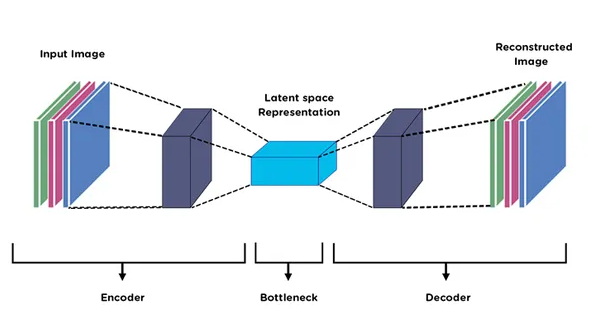
\includegraphics[width=0.7\linewidth]{images/auto_encoder}
		\caption{autoencoder}
		\label{fig:autoencoder}
	\end{figure}

	
	\subsection{Generative Adversarial Network}
	A generator and a discriminator, trained simultaneously through a competitive process. The generator aims to create realistic data, while the discriminator tries to differentiate between real and generated data.
	
	
	
	\section{Text to image models}
	\begin{itemize}
		\item DALL-E
		\item Stable Diffusion
		\item Midjourney
	\end{itemize}
	
	
	
	\newpage
	\section{Foraging Ants}
	\subsection{Model}
	\begin{itemize}
		\item ants wander around on 2D grid:
		\begin{itemize}
			\item starting from nest
			\item avoid obstacles (if any)
			\item follow pheromone gradient (probabilistically)
		\end{itemize}
		\item at current location if not carrying food: pick up a piece of food
		\item if at nest and carrying food: put down food
		\item deposite a unit of pheromone at current location
		\begin{itemize}
			\item "A" if searching for food
			\item "B" if carrying food
		\end{itemize}
		\item Pheromone diffuses and evaporates by constant rate, uniformly across space
	\end{itemize}

	
	\subsection{Ant Colony Optimization (ACO)}
	\begin{itemize}
		\item instead of a grid a graph is used, pheromone is placed on edges
		\item a random starting node is selected
		\item next node is selected probabilistically following edge pheromone gradient
		\item when a solution is found pheromone amounts on path are adjusted: proportionally to quality
		\item the simulation ends when most ants select the same solution 
	\end{itemize}
	
	
	
	\newpage
	\section{The Schelling model}
	An agent-based model of segregation.
	\begin{itemize}
		\item plays on a 2D grid
		\item agents are split into two groups
		\item each agent occupies exactly one tile
		\item each agent has a personal tolerance level in $\left[0,1 \right]$
		\item an agent is happy if:
		\[
		\text{tolerance level} \ge \frac{\text{number of neighbours from the other group}}{\text{number of neighbours}}
		\]
		
		\item if an agent is unhappy it moves to an empty tile
	\end{itemize} 
	
	

	\section{Basic ethical frameworks for technology}
	When you invent a new technology, you uncover a new class of responsibilities. If your invention confers power it starts a race, that without coordination/regulation could result in tragedy.
	
	
	
	\section{Different approaches to machine learning}
	\subsection{Supervised learning}
	In supervised learning we have access to input data and its desired outputs (labels). Our objective is to train a program to generalize the knowledge from our data, so the labels of new data can be predicted.
	
	
	\subsection{Unsupervised learning}
	In unsupervised learning the desired output of our input data is unknown. The goal is to learn the structure of the data, so that it can be clustered/categorized.
	
	\subsection{Reinforcement learning}
	In reinforcement learning an agent learns to make decisions by interacting with an environment. The agent receives feedback in the form of rewards or penalties based on the actions it takes, allowing it to adjust its behaviour in order to optimize strategies over time.
	
	\subsection{Deep learning}
	A subset of machine learning composed of algorithms that permit software to train itself to perform tasks by exposing multilayered neural networks to vast amount of data.


	
	\section{Basic concept of supervised learning}
	Given a training set of $n$ example input/output pairs $(x_1,y_1), (x_2,y_2), \dots, (x_n, y_n)$ (called labelled data), the goal is to approximate the (unknown) function $f$ that maps input vectors to outputs, so that the output of new unlabelled data can be predicted.
	
	\begin{figure}[H]
		\centering
		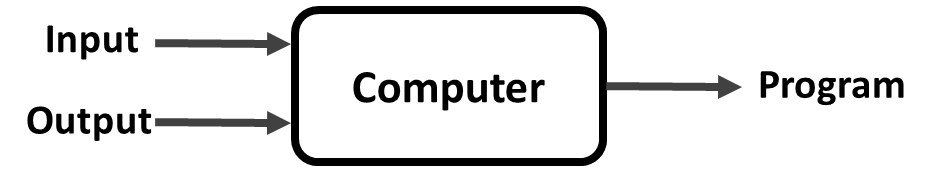
\includegraphics[width=0.7\linewidth]{supervised_learning}
		\caption{Supervised learning}
		\label{fig:supervisedlearning}
	\end{figure}
	
	
	
	\section{Supervised learning by decision trees}
	A decision tree is used to model the mapping between input vectors and decisions (output labels). It is a sequence of tests done starting from the root until a leaf node is reached.
	\\[4pt]
	The simplest kind of decision tree is a boolean decision tree, where each test has a single boolean outcome. This means the entire process can be represented as:
	\[
	OUTPUT \iff \left( Path_1 \lor Path_2 \lor \dots \right)
	\]
	where each path is the conjunction of attribute value tests representing a path from the root to a leaf.
	\\[4pt]
	\noindent
	Most of the time decision tress represent more complex criteria including both discrete and continuous comparisons. 
	\begin{figure}[H]
		\centering
		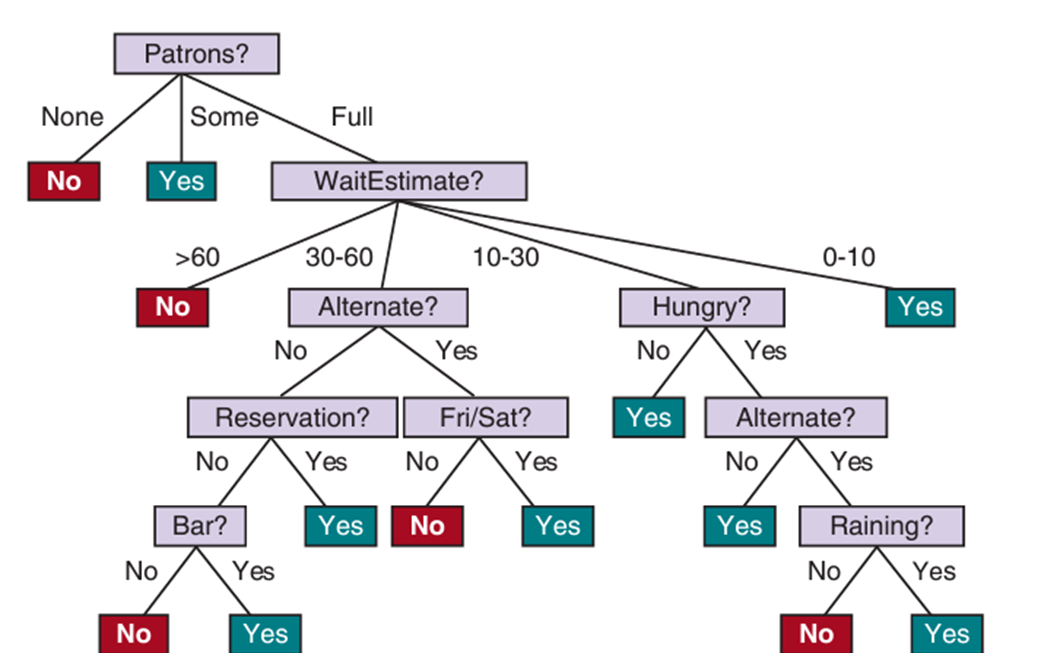
\includegraphics[width=0.7\linewidth]{dec_tree}
		\caption{Decision tree}
		\label{fig:dectree}
	\end{figure}
	
	\newpage
	\subsection{Tree building}
	The decision tree algorithm recursively splits the data into subsets based on the values of different features. At each node of the tree, a decision is made by choosing the feature that best separates the data into distinct classes or reduces the variance in the target variable. The process continues until a stopping criterion is met.
	\begin{figure}[H]
		\centering
		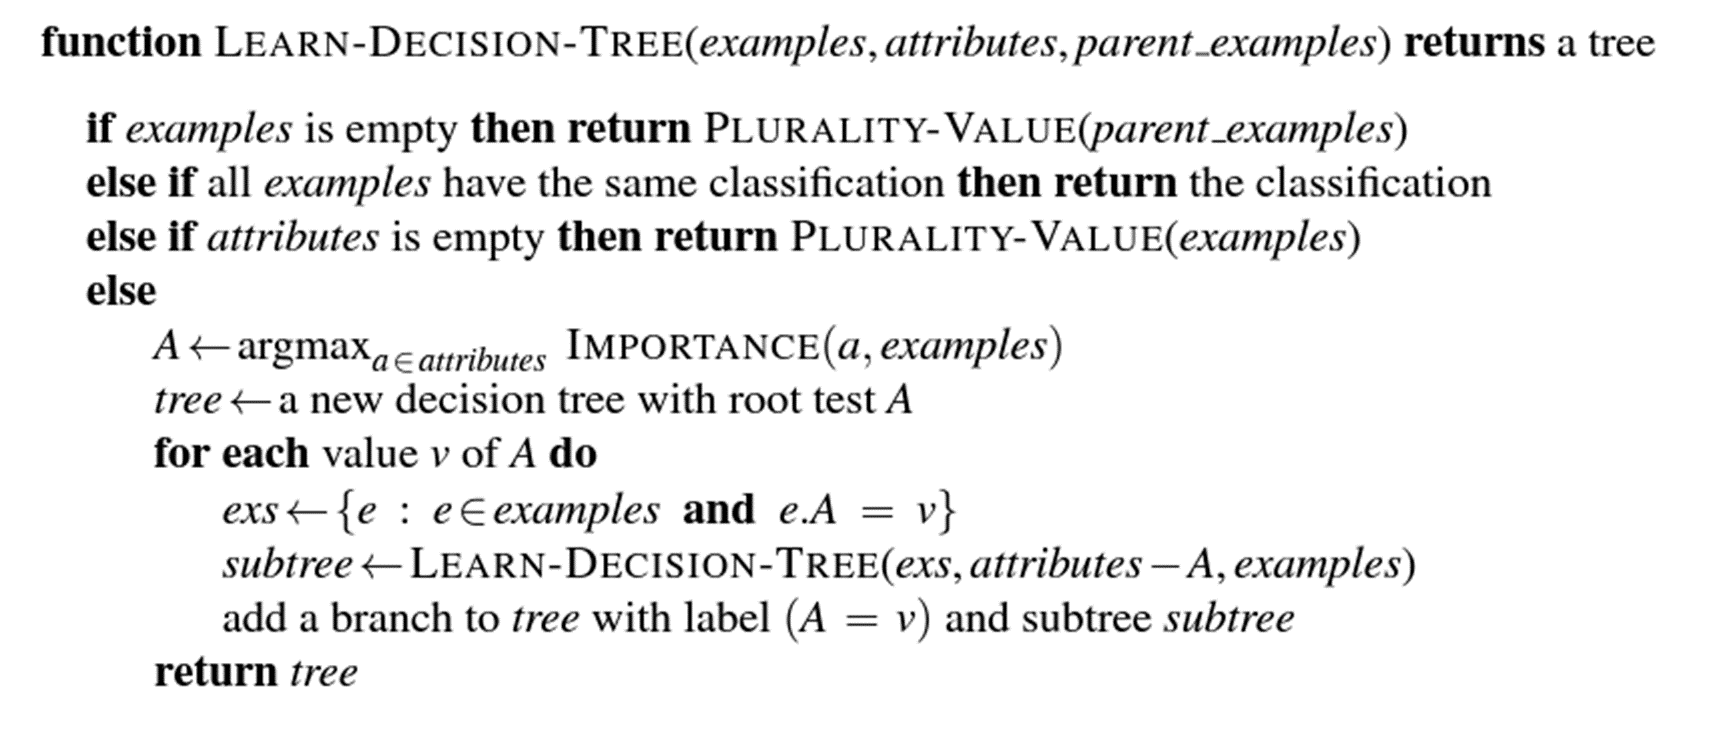
\includegraphics[width=0.7\linewidth]{dec_tree_building}
		\caption{Decision tree building}
		\label{fig:dectreebuilding}
	\end{figure}
	\noindent
	where PLURALITY\_VALUE returns the most common label from a set of data.
	
	\begin{figure}[H]
		\centering
		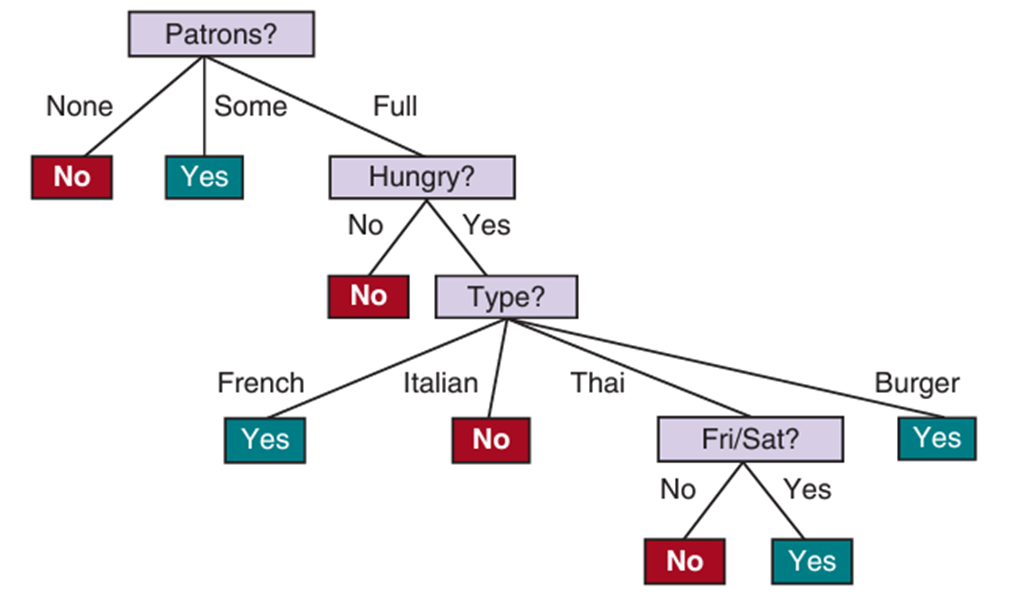
\includegraphics[width=0.7\linewidth]{dec_tree_building2}
		\caption{Decision tree}
		\label{fig:dectreebuilding2}
	\end{figure}
	It is important to note this decision tree has shorter paths and is much simpler than our original tree. The algorithm does not have any knowledge about actual function it merely looks at the examples.
	
	This means the tree is fitted to our training data. This results in decision tress not generalizing well:
	\begin{itemize}
		\item If we increase the number of attributes, overfitting is more likely
		\item If we increase the number of training samples, overfitting is less likely
	\end{itemize}
	
	To improve generalization a technique called pruning is used, during which we examine potentially nodes that only has leaf descendents. If the node appears to be irrelevant it is replaced with a leaf node.
	
	\subsection{Pros}
	\begin{itemize}
		\item Easy to understand
		\item scales well to large data sets
		\item can handle both discrete and continuous inputs
		\item can performing classification and regression
	\end{itemize}
	
	\subsection{Cons}
	\begin{itemize}
		\item Suboptimal accuracy (largely due to the greedy search)
		\item If trees are very deep, making a prediction can be expensive 
		\item decision trees are unstable – adding just one new example can change the entire tree
	\end{itemize}
	
	
	
	\newpage
	\section{Basic concept of unsupervised learning}
	Sometimes we are presented with data without any labels. In some of these cases data may even lock distinguishing characteristics, resulting in manual labelling becoming impossible.
	\noindent
	\\[4pt]
	Unsupervised learning takes a given set of data, and produces output data (labels) and a function, which maps input to output.
	\noindent
	\\[4pt]
	A possible solution to this problem is partitioning data into cluster, groups of highly similar data.
	
	\begin{figure}[H]
		\centering
		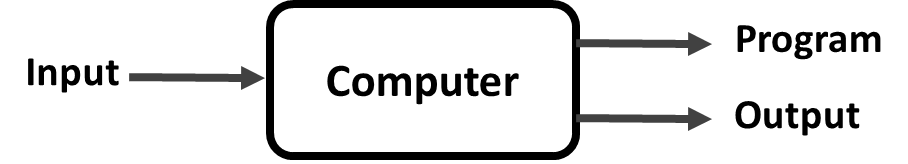
\includegraphics[width=0.7\linewidth]{unsupervised_learning}
		\caption{Unsupervised learning}
		\label{fig:unsupervisedlearning}
	\end{figure}
	
	
	
	\section{k-means algorithm}
	An unsupervised, iterative method for clustering data.
	
	\subsection{Algorithm}
	\begin{enumerate}
		\item define $k$, the number of clusters
		\item initialize $k$ cluster centers at random
		\item repeat:
		\begin{enumerate}
			\item assign each point based on the nearest cluster center
			\item move the center point of each cluster to mean of its members
			\item if no points changed ownership exit
		\end{enumerate}
	\end{enumerate}
	

	\subsection{Example}
	In a wrestling competition, wrestlers are divided into leagues based on their height and weight. Divide the competitors into two leagues ($k=2$) based on the data obtained using the k-means algorithm. Perform the calculation over two iterations, taking the values of the first and second competitors as the initial center points.
	
	\begin{table}[H]
		\centering
		\begin{tabular}{|c|c|c|}
			\hline
			ID & height (cm) & weight(kg) \\ \hline \hline
			1 & 185 & 76 \\ \hline
			2 & 170 & 66 \\ \hline
			3 & 168 & 68 \\ \hline
			4 & 179 & 74 \\ \hline
			5 & 182 & 73 \\ \hline
			6 & 188 & 75 \\ \hline
		\end{tabular}
	\end{table}
	
	\newpage
	\noindent
	First iteration:
	\begin{multicols}{2}		
		\begin{figure}[H]
			\centering
			\begin{tikzpicture}
				\begin{axis}[
					enlargelimits=0.2,
					scatter/classes={
						a={mark=square*,green},
						b={mark=square*,red},
						am={mark=circle*,red},
						bm={mark=circle*,green},
						c={blue}
					}
				]
					\addplot[scatter, mark=*, only marks, scatter src=explicit symbolic,
					nodes near coords*={\Label},
					visualization depends on={value \thisrow{label} \as \Label}
					] table [meta=class] {
						x y class label
						185 76 a 1
						170 66 b 2
						168 68 c 3 
						179 74 c 4
						182 73 c 5 
						188 75 c 6
					};
				\end{axis}
			\end{tikzpicture}
			\caption{Initialize center points}
		\end{figure}
		
		\begin{figure}[H]
			\centering
			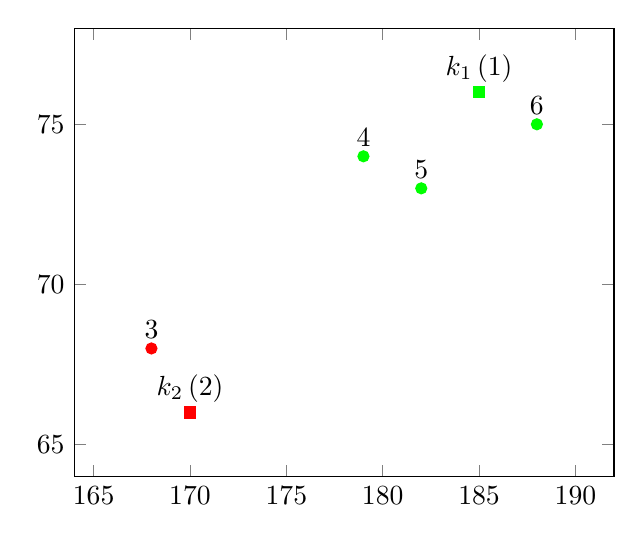
\begin{tikzpicture}
				\begin{axis}[
					enlargelimits=0.2,
					scatter/classes={
						a={mark=square*,green},
						b={mark=square*,red},
						am={red},
						bm={green},
						c={blue}
					}
				]	
					\addplot[
					scatter, mark=*, only marks, scatter src=explicit symbolic,
					nodes near coords*={\Label},
					visualization depends on={value \thisrow{label} \as \Label}
					] table [meta=class] {
						x y class label
						185 76 a $k_1\,(1)$ 
						170 66 b $k_2\,(2)$ 
						168 68 am 3 
						179 74 bm 4
						182 73 bm 5 
						188 75 bm 6
					};
				\end{axis}
			\end{tikzpicture}
			\caption{Assign points to nearest center}
		\end{figure}
	\end{multicols}
	\noindent
	Recalculate center points:
	\begin{align*}
		k_1 &= \left(\frac{185 + 179 + 182 + 188}{4}, \frac{76 + 74 + 73 + 75}{4} \right) = \left(183.5, 74.5 \right) \\
		k_2 &= \left(\frac{170 + 168}{2}, \frac{66 + 68}{2} \right) = \left(169, 67 \right) 
	\end{align*}
	
	\begin{figure}[H]
		\centering
		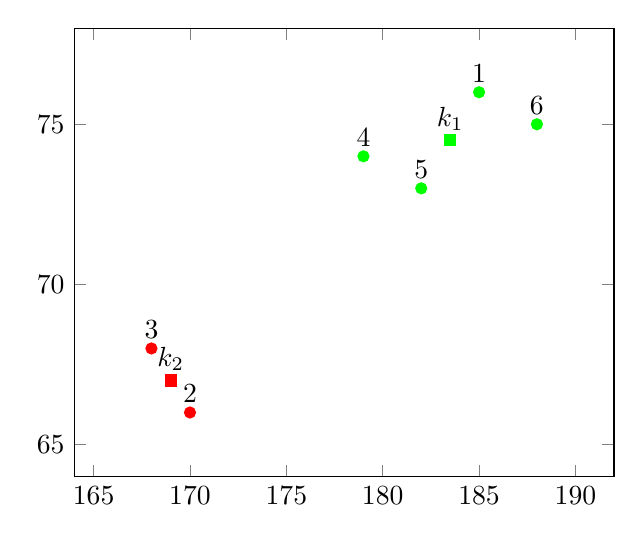
\begin{tikzpicture}
			\begin{axis}[
				enlargelimits=0.2,
				scatter/classes={
					a={mark=square*,green},
					b={mark=square*,red},
					am={red},
					bm={green},
					c={blue}
				}
				]
				
				\addplot[
				scatter, mark=*, only marks, scatter src=explicit symbolic,
				nodes near coords*={\Label},
				visualization depends on={value \thisrow{label} \as \Label}
				] table [meta=class] {
					x y class label
					183.5 74.5 a $k_1$
					169 67 b $k_2$
					185 76 bm 1
					170 66 am 2
					168 68 am 3 
					179 74 bm 4
					182 73 bm 5 
					188 75 bm 6
				};
			\end{axis}
		\end{tikzpicture}
		
		\caption{Move cluster centers}
	\end{figure}
	\noindent
	Second iteration: The points need to be reassigned, based on the new center points. In our case no points change ownership resulting in the termination of the algorithm.
	
	
	
	\newpage
	\section{Mechanism of reinforcement learning}
	Reinforcement learning is a machine learning paradigm where an agent learns to make decisions by interacting with an environment in order to maximize some notion of cumulative reward over time.
	\\[8pt]
	\noindent
	The Markov Decision Process (MDP) which is a mathematical framework that provides a formal way to model decision-making in situations where outcomes are partially random and partially under the control of a decision maker.
	The model contains:
	\begin{itemize}
		\item State Space ($S$): a set of states, representing the possible configurations or situations of the environment
		\item Action Space ($A$): a set of possible actions that the agent can take in each state
		\item Transition Model ($T{(s, a, s’)} \sim \Pr(s’\mid s, a)$): the likelihood of transitioning from state $s$ to $s’$ given a particular $a$ action 
		\item Reward Function ($R$): assigns a numerical value, indicating the immediate reward associated with:
		\begin{itemize}
			\item being in a state ($R(s)$)
			\item taking a specific action in a particular state ($R(s, a)$)
			\item taking an action and ending up in a different state ($R(s, a, s’)$)
		\end{itemize}
		\item Policy ($\pi: S \rightarrow A$): a strategy that specifies the agent's behavior, determining which action to take in each state
	\end{itemize}

	\noindent
	The goal of reinforcement learning is for the agent to learn an optimal policy that maximizes the reward function.
	Both MDPs and reinforcement learning involve the concept of value functions. The state-value function (V) estimates the expected cumulative reward from a given state under a specific policy, while the action-value function (Q) estimates the expected cumulative reward from taking a specific action in a particular state under a specific policy.
	
	
	
	\newpage
	\section{Q-learning method}
	Q-learning is a model-free reinforcement learning algorithm that is used to find the optimal action-selection policy for a given finite Markov decision process. Q-learning is particularly well-suited for problems where the environment is not fully known in advance, and the agent needs to learn by interacting with the environment.
	
	\begin{figure}[H]
		\centering
		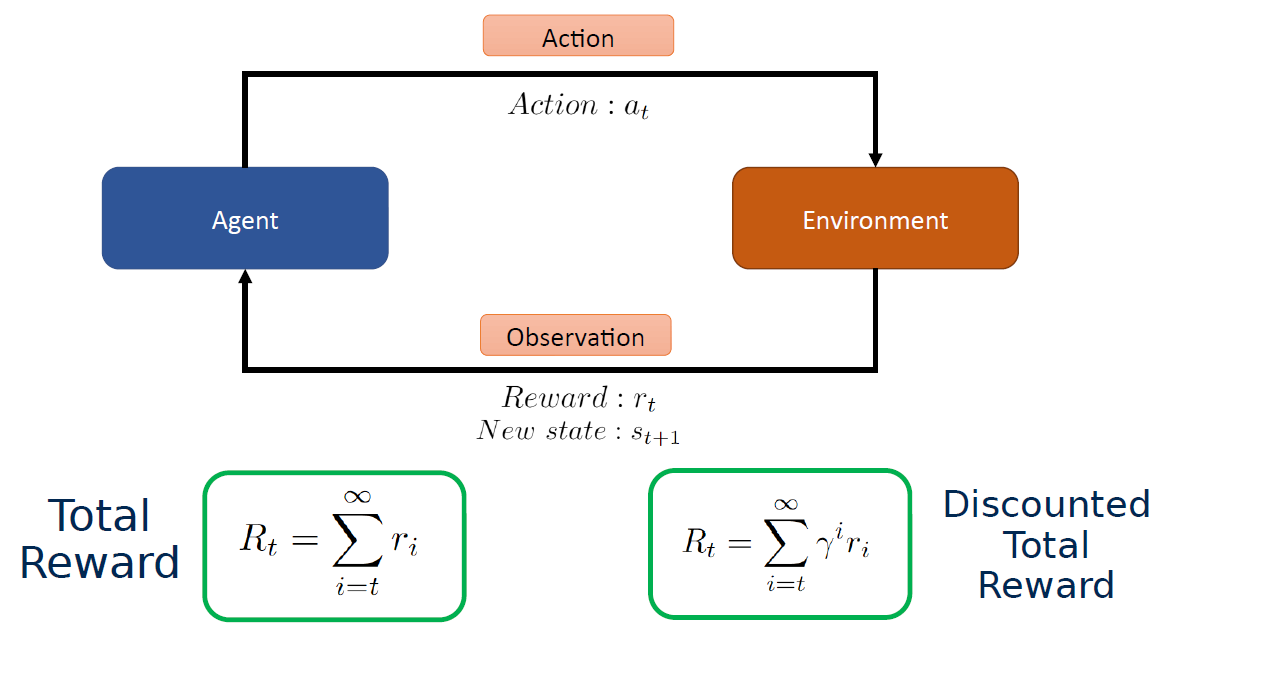
\includegraphics[width=0.7\linewidth]{q_learning}
		\caption{Q-learning}
		\label{fig:qlearning}
	\end{figure}
	\noindent
	Key concepts and components of Q-learning:
	\begin{itemize}
		\item State (S) and Action (A): The environment is represented as a set of states (S) and a set of possible actions (A). The agent interacts with the environment by taking actions at different states
		\item Q-Values (Q(s, a)): Q-values are used to represent the expected cumulative reward of taking a particular action in a specific state and following the optimal policy thereafter.
		\item Q-Table: In Q-learning, a Q-table is used to store Q-values for all state-action pairs. Initially, the Q-table is filled with arbitrary values, and the agent updates these values as it interacts with the environment.
		\item Learning Iteration: The agent iteratively interacts with the environment, updates the Q-values using the Bellman equation, and refines its policy over time.
	\end{itemize}
	\noindent
	Downsides of Q-learning:
	\begin{itemize}
		\item Cannot handle continuous action spaces
		\item Policy is deterministically computed from the Q function by maximizing the reward, so the model cannot learn stochastic policies
	\end{itemize}
	
	
	
	\newpage
	\section{Deep Learning methods, value learning and policy learning}
	Deep learning algorithms can be classified based on their strategy for finding the optimal policy ($\pi^*$).
	
	\subsection{Value learning}
	The optimal policy is derived from a learned function $Q$ called the value function. The optimal policy is always choosing the best possible action in every state:
	\[
	\pi^*(s) = \argmax_{a}{Q(s,a)}
	\]
	
	\subsection{Policy learning}
	In policy learning, the goal is to directly learn the optimal policy without explicitly estimating the value function. It estimates the policy using a parameterized function, which is fine tuned through a learning process.
	\[
	\pi^*(s) \sim \pi(s)
	\]
	
	
	
	\section{Policy gradient algorithm}
	The training algorithm of a policy is the following:
	\begin{enumerate}
		\item Initialize the agent
		\item Run the policy until termination:
		\begin{enumerate}
			\item Record all states, actions, rewards
			\item Decrease probability of actions that resulted in low reward
			\item Increase probability of actions that resulted in high reward
		\end{enumerate}
	\end{enumerate}
	
	
	
	\newpage
	\section{Basic concept of evolutionary algorithms}
	Evolutionary algorithms are stochastic search methods that computationally simulate the natural evolutionary process using the concept of the survival of the fittest.
	\begin{itemize}
		\item Gene: functional entity that encodes a specific feature of the individual (e.g. hair color)
		\item Allele: value of gene (e.g. blonde)
		\item Genotype: the specific combination of alleles carried by an individual
		\item Phenotype: the physical makeup of an organism
		\item Locus: position of the gene within the chromosome
		\item Individual (chromosome): represents an encoded (binary or real) candidate solution for the problem
		\item Population: collection of individuals currently alive
	\end{itemize}
	
	
	
	\section{Optimization by genetic algorithm}
	A genetic algorithm is a population-based stochastic optimization method inspired by natural selection. It utilizes three operators inspired by biology: selection, crossover and mutation.
	\\[4pt]
	\noindent
	The individuals are evaluated according to some criterion called the fitness function on how good of a solution they can provide to the given problem. Better individuals have a higher fitness value, thus they have a higher chance to survive.
	
	
	\subsection{Selection}
	There are many ways to select chromosomes to survive to the next generation. One such method is roulette wheel selection (also known as fitness proportionate selection), where the chance of selecting an individual is proportionate to its fitness value.
	
	\[
	\text{expected count in crossover} = \frac{\text{fitness of individual}}{\text{total fitness of population}} \cdot \text{size of population}
	\]
	
	\subsection{Crossover}
	A random locus is selected. The tails after the locus are exchanged.
	\begin{figure}[H]
		\centering
		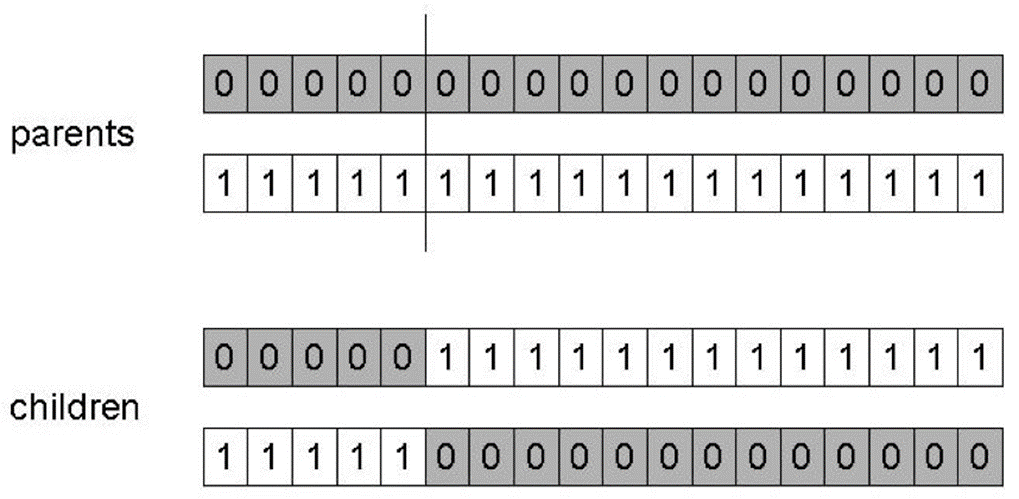
\includegraphics[width=0.7\linewidth]{crossover}
		\caption{Crossover}
		\label{fig:crossover}
	\end{figure}
	
	\subsubsection{Alternative crossover operators}
	\begin{figure}[H]
		\centering
		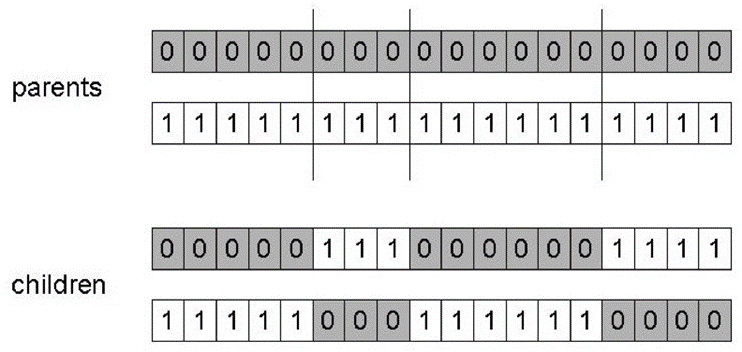
\includegraphics[width=0.7\linewidth]{npoint_cross}
		\caption{n point crossover}
		\label{fig:npointcross}
	\end{figure}
	
	\begin{figure}[H]
		\centering
		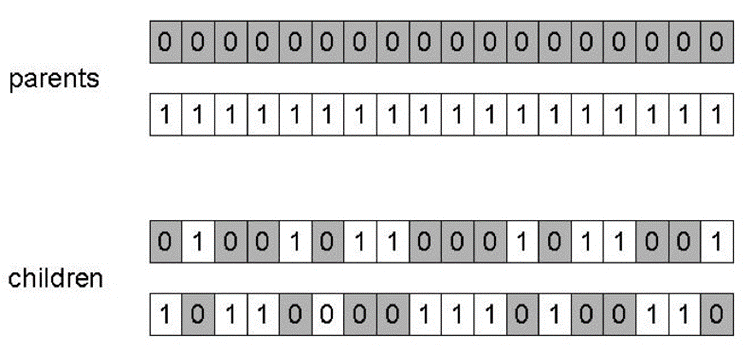
\includegraphics[width=0.7\linewidth]{uniform_cross}
		\caption{uniform crossover}
		\label{fig:uniformcross}
	\end{figure}
	
	
	\subsection{Mutation}
	Each gene has a chance to change with a $p_m$ probability called the mutation rate.
	\begin{figure}[H]
		\centering
		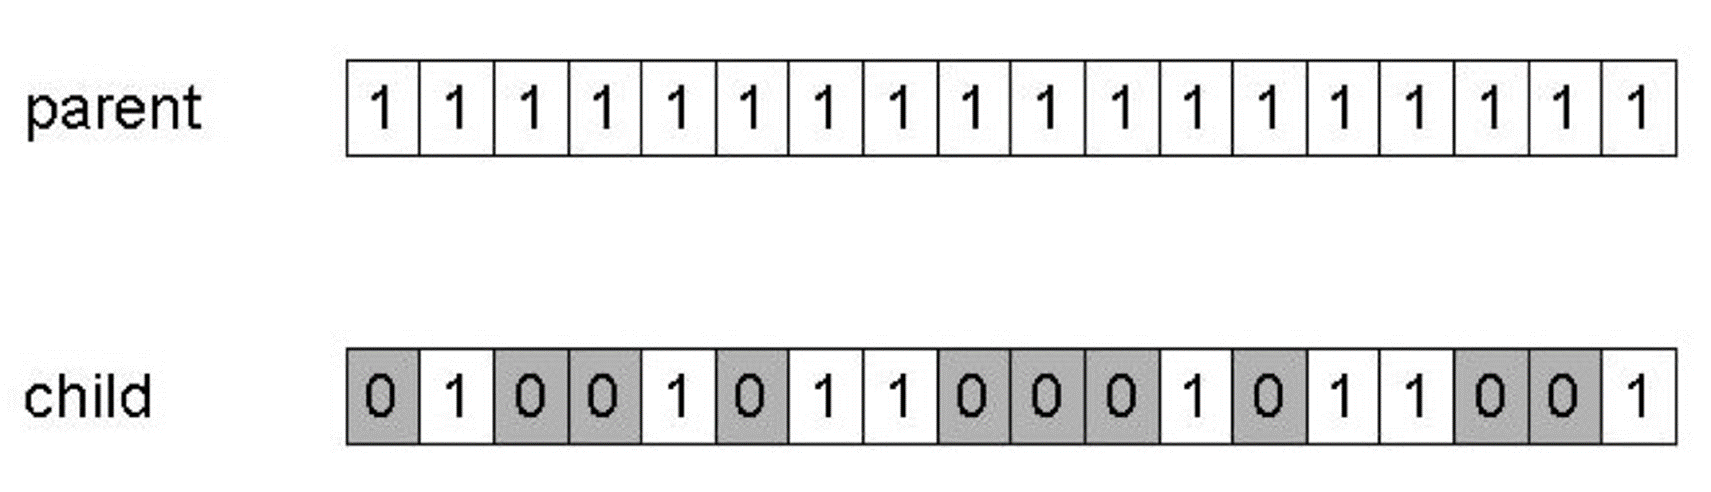
\includegraphics[width=0.7\linewidth]{mutation}
		\caption{Mutation}
		\label{fig:mutation}
	\end{figure}
	
	
	\newpage
	\subsection{Example}
	Find $x^2$ over $ \left\lbrace 0,1,\dots,31 \right\rbrace $! 	
	\begin{figure}[H]
		\centering
		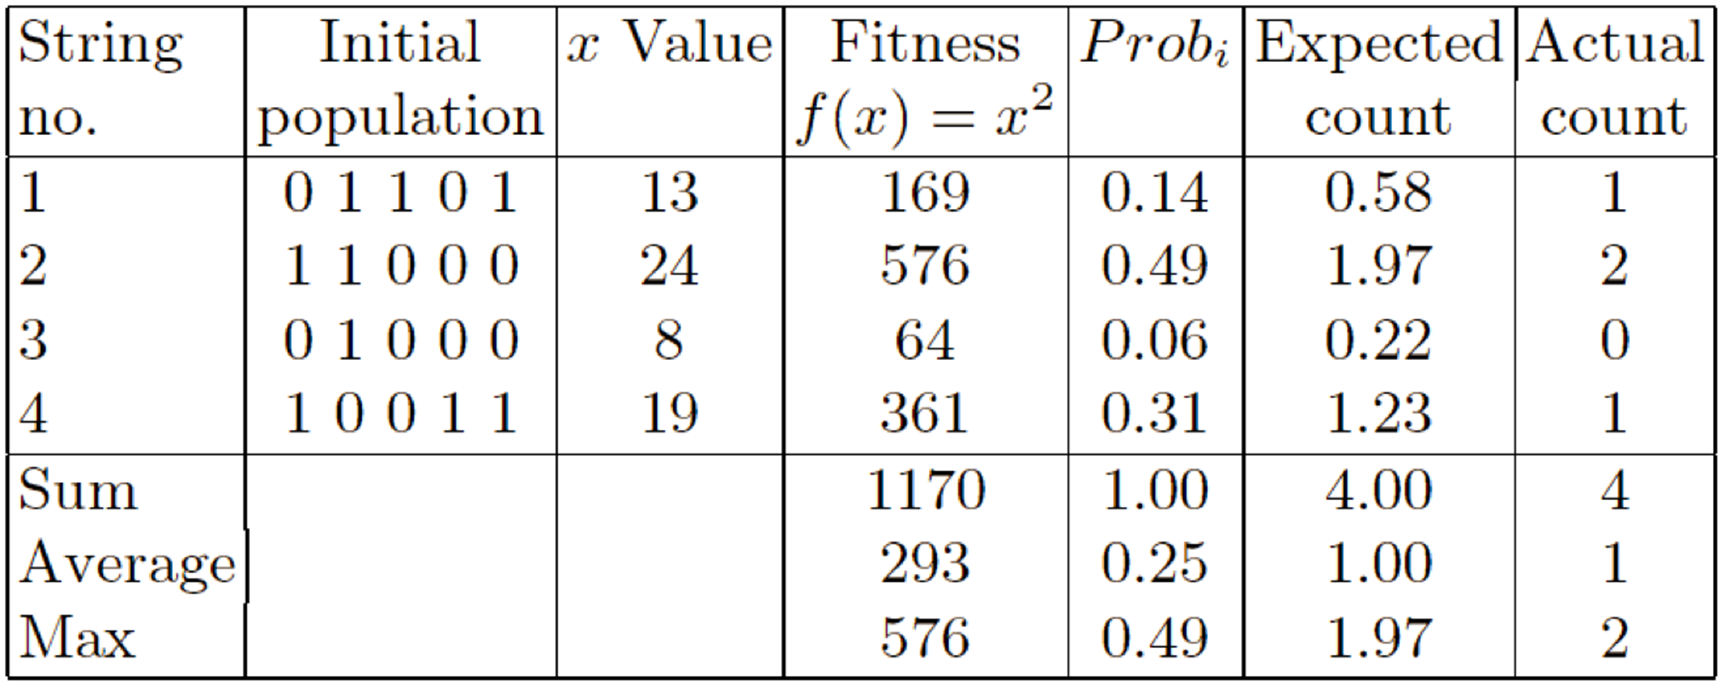
\includegraphics[width=0.7\linewidth]{goldberg_selection}
		\caption{Selection}
		\label{fig:goldbergselection}
	\end{figure}
	
	\begin{figure}[H]
		\centering
		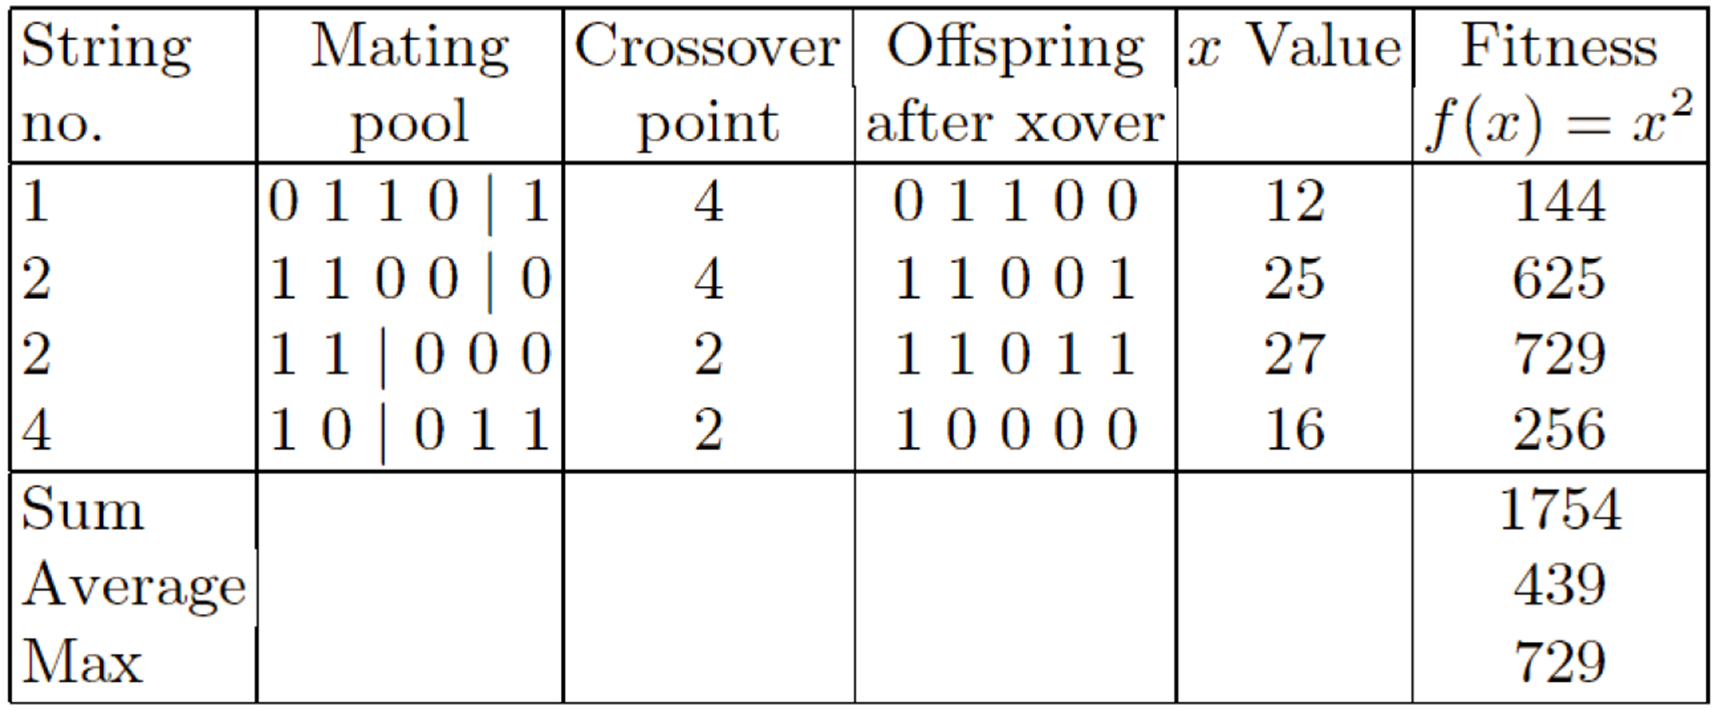
\includegraphics[width=0.7\linewidth]{goldberg_crossover}
		\caption{Crossover}
		\label{fig:goldbergcrossover}
	\end{figure}
	
	\begin{figure}[H]
		\centering
		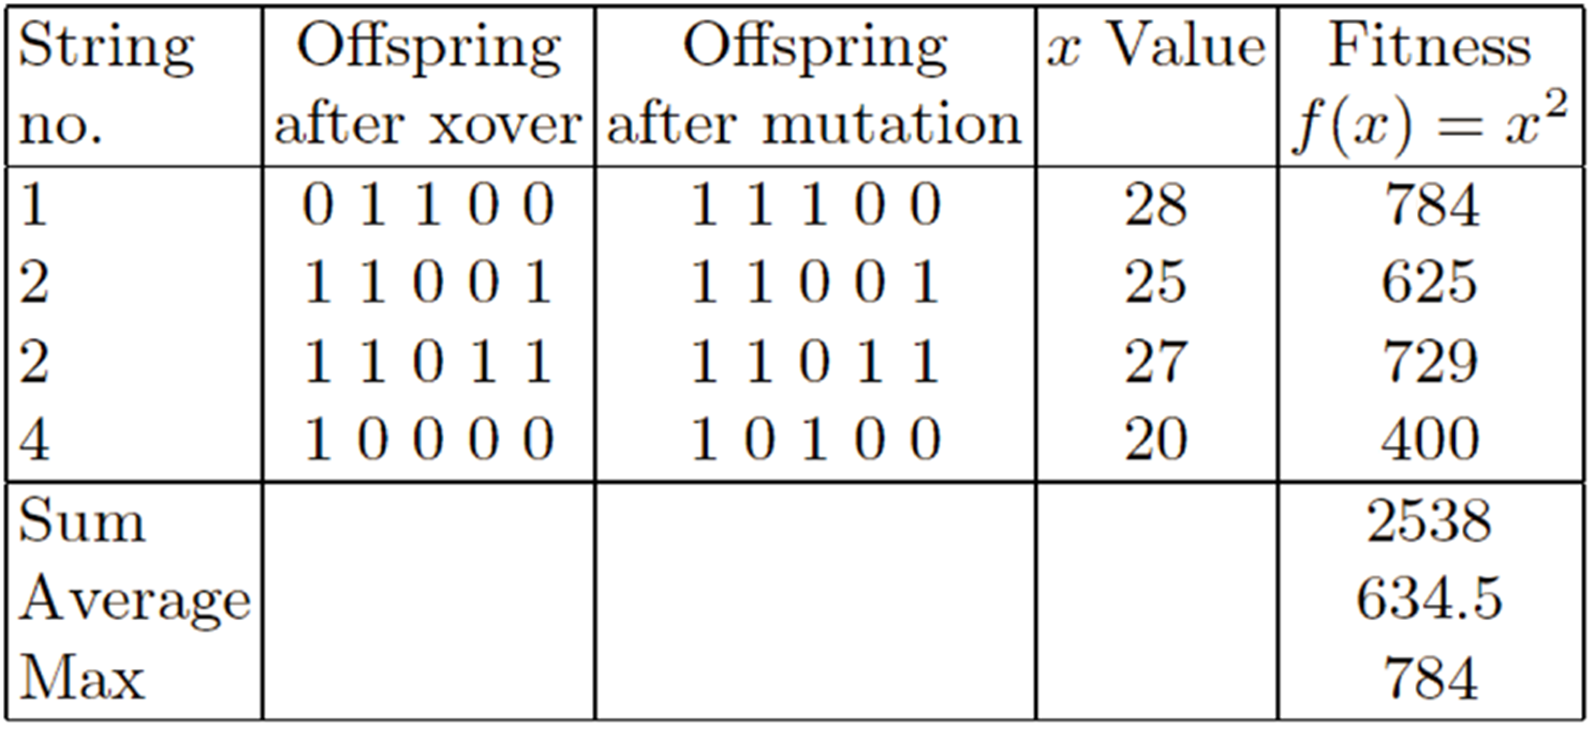
\includegraphics[width=0.7\linewidth]{goldberg_mutation}
		\caption{Mutation}
		\label{fig:goldbergmutation}
	\end{figure}
	
	
	
	\newpage
	\section{Basic concept of genetic programming, differences with genetic algorithms}
	Genetic programming applies the approach of genetic algorithm to the space of possible computer programs, allowing the generation of syntactically valid and executable programs.
	\\[4pt]
	\noindent
	This way each individual becomes an expression tree representing a syntactically valid executable program.
	
	\begin{figure}[H]
		\centering
		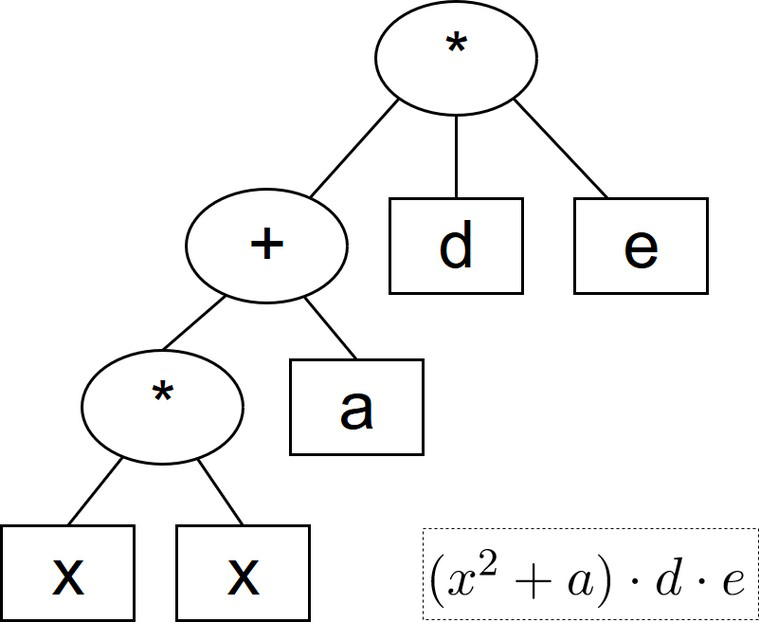
\includegraphics[width=0.3\linewidth]{images/expr_tree}
		\caption{Expression tree}
		\label{fig:exprtree}
	\end{figure}
	\noindent
	The approach requires the definition of the following:
	
	\begin{itemize}
		\item set of terminals (foo, bar, x, y, i)
		\item set of functions (+, -, IF, \%)
		\item the fitness measure 
		\item the parameters for the run
		\item the criterion for terminating a run
	\end{itemize}
	
	\subsection{Selection (reproduction)}
	\begin{itemize}
		\item select parent based on fitness
		\item copy it without any change into the next generation of the population
	\end{itemize}
	
	 
	\subsection{Mutation}
	\begin{itemize}
		\item select 1 parent (based on fitness)
		\item pick a point in the tree
		\item replace the subtree at the picked point with a new subtree generated the same way as trees in the initial population
		\item put the offspring into the next generation of the population 
	\end{itemize}
	
	
	\subsection{Crossover}
	\begin{itemize}
		\item select 2 parents (based on fitness)
		\item randomly pick a node in the tree for first parent
		\item independently randomly pick a node for second parent
		\item exchange the subtrees at the two picked points
		\item put the offspring into the next generation of the population
	\end{itemize}
	
	
	
	\newpage
	\section{The basic concept of swarm intelligence}
	A collective system capable of performing complex tasks in a dynamic and changing environment without any external control or central coordination. Capable of achieving a collective performance that cannot normally be achieved by the organism alone.

	\begin{itemize}
		\item Distributed, massively parallel (many agents)
		\begin{itemize}
			\item Individual agents are simple and disposable (cheap)
			\item Typically partially stochastic (i.e., non-deterministic)
		\end{itemize}
		\item Intelligence is optimising or performing a task
		\begin{itemize}
			\item Stochastic: approximations, different runs may give slightly different results
			\item Typically continuous optimisation / performance of a series of tasks
		\end{itemize}
		\item Robust:
		\begin{itemize}
			\item Adapts to changing environments (and performs well)
			\item Graceful degradation: withstands removal of agents (potentially many of them)
		\end{itemize}
	\end{itemize}
	
	
	
	\section{Optimization by Particle Swarm Optimization}
	PSO applies the concept of social interaction to problem solving. Particles move in swarms in search of the best solution. Each particle is a spatial point that adjusts its flight based on experience gained by itself and by its peers. This way particles will converge towards the optimal solution.
	
	\begin{itemize}
		\item pbest: best solution achieved by the particle
		\item gbest: best solution achieved by the swarm 
	\end{itemize}
	
	\noindent
	Each particle changes its position based on the following information: 
	\begin{itemize}
		\item current position
		\item current velocity
		\item distance between current position and pbest
		\item distance between current position and gbest
	\end{itemize}
	
	
	
	\newpage
	\section{Recent swarm intelligence techniques}
	\subsection{Firefly}
	\begin{itemize}
		\item similar to Particle Swarm Optimization
		\item particles are fireflies who emit light
		\item light intensity reduces over distance and respects absorption ($\gamma$)
		\item brightness depends on how good of a solution they provide:
			\[
				(I_0, d, \gamma) = I_0 \cdot e^{-\gamma d^2}
			\]
			where $d$ is a distance metric and $I_0$ is the individuals light intensity at 0 distance
		\item each individual moves towards brighter fireflies and also do some random movement
	\end{itemize}
	
	\subsubsection{Special cases}
	\begin{itemize}
		\item $\gamma = 0$ clear air, all fireflies can see each other
		\item $\gamma = \infty $ foggy air, fireflies can't see each other result in random walk
	\end{itemize}
	
	\subsection{Grey wolf}
	\href{https://en.wikiversity.org/wiki/Algorithm_models/Grey_Wolf_Optimizer}{\color{blue}{GWO algorithm}}
	
	

	
	\newpage
	\section{Basics of neural networks}
	The fundamental cellular unit of nervous system is called neuron. A neuron is a simple processing unit connected to approximately 1000 neurons. The function of a neuron is receiving and combining signals from other neurons through input paths called dendrites. If the combined input signal is strong enough, the neuron fires and produces an output signal and sends the output along the axon to other neurons.
	\\[8pt]
	\noindent
	An artificial neuron is a mimic of a biological neuron.
	
	\begin{figure}[H]
		\centering
		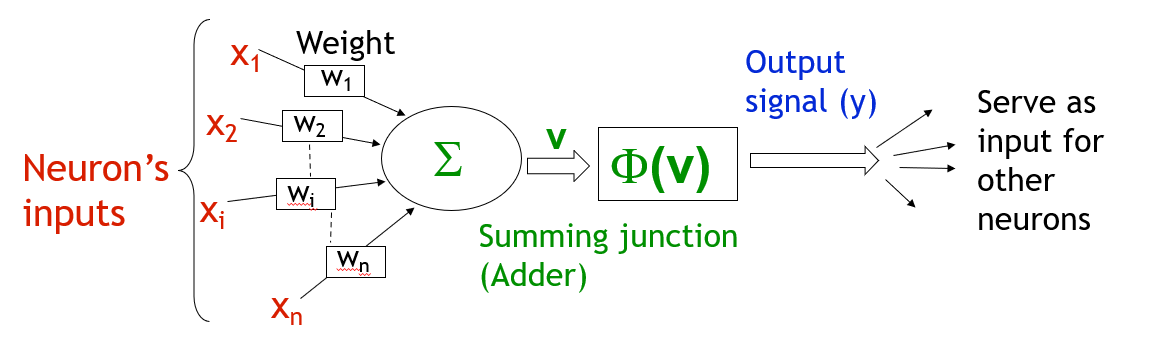
\includegraphics[width=0.7\linewidth]{artifical_neuron}
		\caption{Artificial neuron}
		\label{fig:artificalneuron}
	\end{figure}
	
	A single neuron is unable to solve complex problem, however an interconnected system of neurons can deliver complex behaviour. $\Phi$ is the activation function responsible for keeping the values in given range.
	
	\section{Perceptron, Perceptron training}
	\subsection{Definition}
	The perceptron is an supervised algorithm for learning a binary classifier called a threshold function. A (single-layer) perceptron is only capable of learning linear threshold functions. In the context of neural networks, a  perceptron is an artificial neuron using the Heaviside step function as the activation function. 
	
	Multilayer perceptron also exist which are capable of separating linearly inseparable variables as well.
	
	
	\subsection{Training}
	
	\begin{enumerate}
		\item Initialization
		\begin{itemize}
			\item set the initial weights
			\item set the threshold $\theta$ to a random number in $\left[ -0.5, 0.5 \right] $
			\item set the learning rate $\mu$ to a positive value less than 1
		\end{itemize}
		\item Activation (calculate actual output of at iteration)
		\item Weight learning (update weights based on output)
		\item Iteration (repeat steps 2-4 until convergence)
	\end{enumerate}
	
	\section{Basic concept of CRISP-DM}
	An open standard process model that describes common approaches used by data mining experts, that breaks the process of data mining into six major phases:
	\begin{enumerate}
		\item Business Understanding
		\item Data Understanding
		\item Data Preparation
		\item Modelling
		\item Evaluation
		\item Deployment
	\end{enumerate}
\end{document}
